\scanpage{81}

$f$ fonction convexe sur l'ouvert convexe $U$,

\[
(x,y)\in G_f\iff x\in U\text{ et } y>f(x)
\]

Soit \deleted{\unsure{$x,y$|$x_i,y_i$}} $(a,b)$ avec $b=f(a)$ $(a\in U)$, \deleted{\unsure{on|donc}} soit $H$ un hyperplan passant par $(a,b)$ ne rencontrant pas l'ouvert $G_f$, alors : 1) il est de la forme

\[
y-b=\deleted{\unsure{\sum c_i x_i+\beta}}=\sum c_i(x_i-a_i)
\]

(car ne \unsure{contient} pas la droite $x=a$), soit $y=L_a(x)$

2) On a $f(x)\geq L(x)$ pour \uline{\unsure{tout}} $x\in U$ (en effet, l'un des deux \deleted{\unsure{hyperplans}} $\frac12$ espaces \inserted{ouverts} déterminés par $H$ contient $G_f$, et ce ne peut être que celui donné par $y>L(x)$. \deleted{\unsure{donc}} d'où la conclusion).

3) On a pour $x\in E$ $f(x)=\sup_a L_a(x)$ (le sup étant obtenu), et réciproquement.

4) Si au point $a$, $f(x)$ est croissante alors les $c_i$ sont $\geq0$. En effet, si on avait p. ex $c_1<0$, alors $f(x_1,a_2,\ldots a_n)$ est croissante au point $x_1=a_1$,

\figure{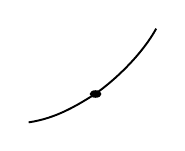
\begin{tikzpicture}[x=1cm,y=1cm]\draw[line width=.7pt] (0,0) .. controls (.35,.05) and (.62,.22) .. (.83,.35) .. controls (1.12,.55) and (1.45,.88) .. (1.62,1.19);\fill (.85,.36) ellipse (.075 and .048);\end{tikzpicture}}

et \deleted{de} minorée par $L(x_1,a_2,\ldots a_n)$, fonction linéaire prenant au point $a$ la même valeur que $f$. Cette dernière ne peut être strictement décroissante car on aurait $f(x_1)\leq f(a)\leq\unsure{\underline{f}|L|f}(x_1)$ pour $x_1<a_1$ voisin de $a_1$.

% archive sheet number: 82
